
\section{Introduction}

The acquisition of labeled training data represents one of the most significant bottlenecks in developing robust object detection systems. Manual annotation of real-world imagery is time-consuming, expensive, and often fails to capture the full distribution of scenarios that a deployed model may encounter. Synthetic data generation has emerged as a compelling solution to these challenges, offering the ability to produce unlimited quantities of perfectly labeled training images with precise control over scene parameters. This chapter provides a comprehensive treatment of synthetic data generation frameworks, the complete taxonomy of tunable parameters, priority rankings based on empirical evidence, and end-to-end pipeline architectures for training object detection models.

The fundamental premise underlying synthetic data generation is that computer-generated imagery, when properly configured, can serve as an effective proxy for real-world training data. Research has demonstrated that models trained exclusively on synthetic data can achieve mAP@50 scores exceeding 0.91 when evaluated on real-world test sets, particularly when domain randomization techniques are employed to bridge the simulation-to-reality gap. The key insight from the domain randomization literature is that by exposing the neural network to sufficient variation during training, the real world appears as merely another sample from the training distribution.

This chapter is organized as follows. Section~\ref{sec:frameworks} surveys the major synthetic data generation frameworks, comparing their capabilities, strengths, and appropriate use cases. Section~\ref{sec:parameter_taxonomy} presents an exhaustive taxonomy of tunable parameters organized by category, with typical ranges and implementation considerations. Section~\ref{sec:priority_ranking} provides an evidence-based ranking of parameter importance derived from ablation studies in the literature. Finally, Section~\ref{sec:pipeline_architecture} describes complete generation pipeline architectures including annotation format generation and quality control measures.

\begin{figure}[htbp]
\centering
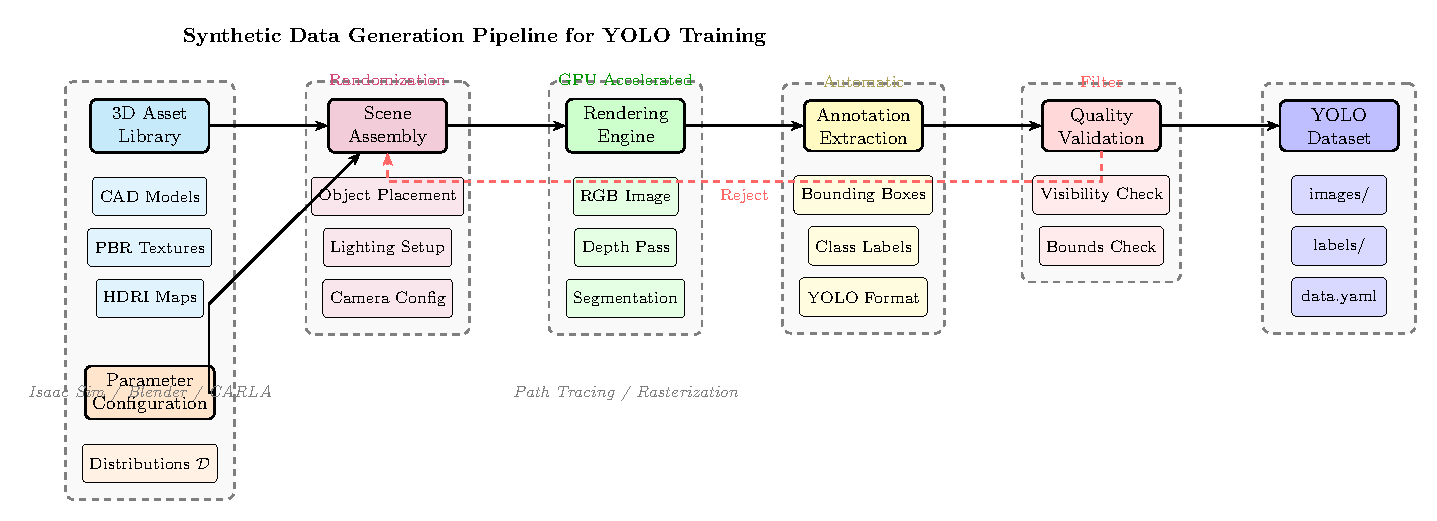
\includegraphics[width=\textwidth]{figures/ch04_fig1_sdg_pipeline.pdf}
\caption{End-to-end synthetic data generation pipeline for YOLO training. The pipeline encompasses six major stages: input preparation (3D assets and parameter configuration), scene assembly with domain randomization, GPU-accelerated rendering, automatic annotation extraction in YOLO format, quality validation with rejection loops, and final dataset output. Each stage is color-coded to indicate its primary function, with dashed arrows showing the rejection feedback loop for failed samples.}
\label{fig:sdg_pipeline}
\end{figure}

\section{Synthetic Data Generation Frameworks}
\label{sec:frameworks}

The landscape of synthetic data generation tools encompasses both general-purpose rendering engines and specialized simulation platforms designed specifically for machine learning applications. This section provides detailed descriptions of the major frameworks, their architectural approaches, and guidance for framework selection.

\subsection{NVIDIA Omniverse and Isaac Sim}

NVIDIA Isaac Sim represents the current state-of-the-art in synthetic data generation for robotics and computer vision applications. Built upon the NVIDIA Omniverse platform, Isaac Sim provides a comprehensive suite of tools for generating photorealistic imagery with precise ground truth annotations. The platform leverages NVIDIA's RTX technology for hardware-accelerated ray tracing, enabling the generation of physically accurate lighting, reflections, and shadows that closely approximate real-world optical phenomena.

The core synthetic data generation capability within Isaac Sim is provided through the Omniverse Replicator extension. This extension implements a domain-specific language for defining randomization distributions over scene parameters, enabling researchers to specify stochastic, controlled, and bounded parameter variations. The Replicator generates data in simulation rather than requiring real-world collection, automatically producing labels that can be directly consumed by training pipelines. This eliminates the preprocessing steps typically required when working with manually annotated datasets.

Isaac Sim's synthetic data generation capabilities span multiple approaches depending on the application requirements. Scene-based generation involves constructing complete 3D environments with semantically meaningful object placements, while object-based generation focuses on capturing individual objects from multiple viewpoints against varied backgrounds. Environment-based generation leverages procedurally generated worlds from tools like Infinigen to create diverse outdoor scenes. The platform also supports pose estimation synthetic data generation, implementing domain randomization techniques inspired by NVIDIA's research on the MESH and DOME datasets.

A distinguishing feature of Isaac Sim is its integration with SimReady assets, which are OpenUSD-based 3D models with built-in semantic labeling, dense captions, and physics properties based on USDPhysics. These assets streamline the simulation setup process by providing ready-to-use models with appropriate physical properties for realistic scene dynamics. The SimReady Warehouse 01 Assets Pack, for example, includes extensive collections of industrial objects such as pallets, storage racks, and ramps that are immediately usable for warehouse robotics applications.

Practical applications of Isaac Sim have demonstrated impressive results. One notable case study involved training a deep neural network to detect forklifts for collision avoidance with autonomous mobile robots, generating over 90,000 training images. Another application generated a synthetic dataset of 5,000 images for pallet jack detection in warehouse environments, applying domain randomization to pallet jack colors, poses, and camera positions while varying lighting and object placement.

\subsection{Blender with Python Scripting}

Blender represents a highly accessible and flexible option for synthetic data generation, combining professional-grade 3D rendering capabilities with extensive Python scripting support. As an open-source application licensed under the GNU General Public License, Blender eliminates licensing costs while providing rendering quality comparable to commercial alternatives. The Python API enables complete automation of scene construction, object manipulation, and batch rendering operations.

Blender offers two primary rendering engines with distinct performance and quality characteristics. The Cycles engine implements unbiased path tracing, simulating realistic light transport through the scene by tracing rays from the camera through multiple bounces until they reach light sources. This approach accurately captures global illumination effects including indirect lighting, color bleeding, and caustics. Research has demonstrated that path tracing consistently outperforms rasterization-based rendering across object detection benchmarks, with performance differences ranging from 0.3\% to 5.1\% mAP@50 depending on the specific use case. The Eevee engine provides real-time rasterization-based rendering that executes substantially faster but produces less physically accurate results.

\begin{figure}[htbp]
\centering
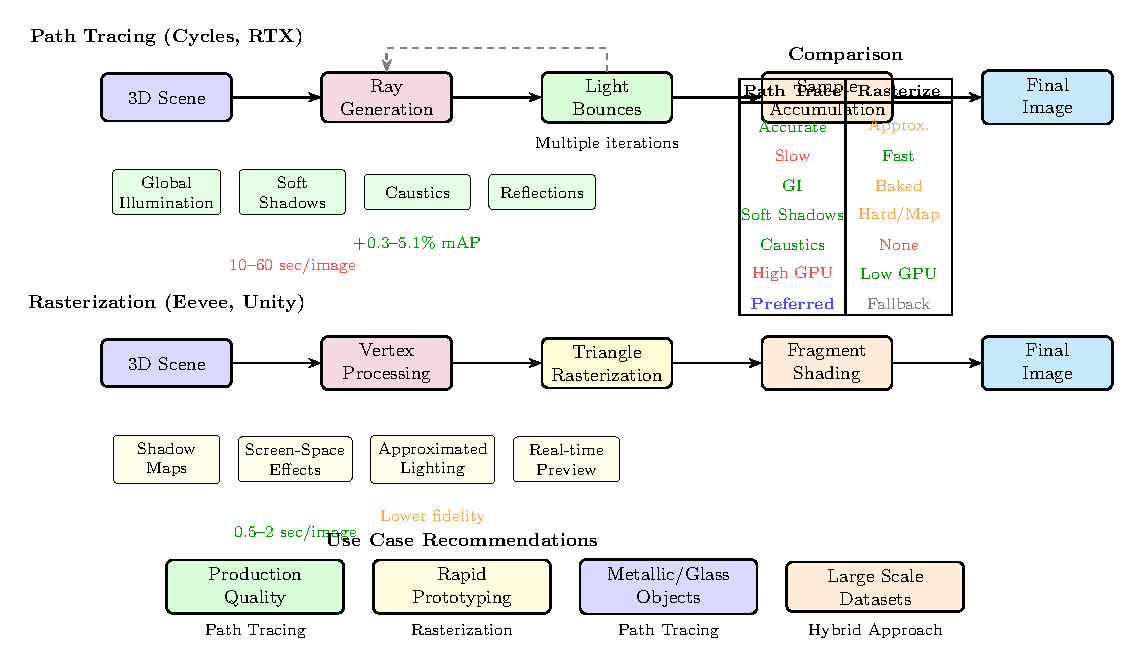
\includegraphics[width=\textwidth]{figures/ch04_fig3_rendering_comparison.pdf}
\caption{Comparison of path tracing and rasterization rendering pipelines for synthetic data generation. Path tracing (top) simulates realistic light transport through multiple bounces, producing physically accurate global illumination, soft shadows, and caustics at the cost of longer render times (10--60 seconds per image). Rasterization (bottom) uses projection and fragment shading for real-time preview speeds (0.5--2 seconds per image) with approximated lighting effects. The comparison table and use case recommendations guide practitioners in selecting the appropriate rendering approach for their application requirements.}
\label{fig:rendering_comparison}
\end{figure}

Several Python libraries extend Blender's capabilities specifically for synthetic data generation. The Starfish library, developed for spacecraft pose estimation, provides utilities for generating long sequences of synthetic images with intuitive parameter specifications. Starfish includes an annotation module with utility functions for generating segmentation masks using Blender's ID Mask Node system. Other notable libraries include BlenderProc, which implements a modular pipeline for synthetic data generation with support for common annotation formats.

A typical Blender-based synthetic data pipeline involves programmatically loading 3D object models, randomizing their positions, rotations, and scales, configuring lighting and camera parameters, rendering the scene to an image file, and extracting ground truth annotations from the scene graph. The bpy module provides access to all Blender functionality from Python, enabling scripts to modify virtually any aspect of the scene. Ground truth extraction leverages Blender's ability to render object indices into auxiliary passes, which can then be processed to generate bounding boxes, segmentation masks, or keypoint annotations.

\subsection{Infinigen Procedural Generation}

Infinigen represents a paradigm shift in synthetic data generation through its entirely procedural approach. Developed by the Princeton Vision and Learning Lab and presented at CVPR 2023, Infinigen generates all scene content from randomized mathematical rules without relying on any external assets or scanned geometry. This procedural foundation enables infinite variation at both the object and scene levels, as each generation produces genuinely novel content rather than sampling from a fixed asset library.

The system covers a broad range of natural world content including procedurally generated plants, animals, terrains, and natural phenomena such as fire, clouds, rain, and snow. Each category of content is defined by mathematical functions that capture the essential characteristics of the object class while admitting substantial variation through parameter randomization. A procedurally generated tree, for example, follows botanical growth rules that produce realistic branching structures, bark textures, and leaf distributions, yet each generated instance is unique.

Infinigen Indoors, presented at CVPR 2024, extends the system to indoor environments by introducing procedural generators for furniture, architectural elements, appliances, and everyday objects. The indoor extension also introduces a constraint-based arrangement system with a domain-specific language for expressing diverse constraints on scene composition. This enables the generation of semantically coherent room layouts where objects are placed according to functional relationships rather than purely random positioning.

The ground truth outputs from Infinigen are comprehensive, including RGB imagery, metric depth maps, surface normals, occlusion boundaries, pixel-level semantic and instance segmentation, 3D bounding boxes, optical flow, and per-object semantic labels. These outputs are exported in standard formats including PNG, EXR, JSON, and NPZ for direct consumption by training pipelines. For embodied agent training, Infinigen provides export to URDF, USD, and MJCF formats that can be directly loaded into real-time simulators such as Omniverse, Unreal Engine, and MuJoCo.

\subsection{Unity Perception}

Unity Perception was developed by Unity Technologies as a toolkit for generating synthetic datasets for perception-based machine learning tasks. The package provided tools for object detection, semantic segmentation, pose estimation, and related computer vision applications. The system was integrated into the Unity game engine, leveraging Unity's mature 3D rendering pipeline and extensive asset ecosystem.

The Perception package architecture centered on the Perception Camera component, which captured synthetic sensor data from simulated cameras within the Unity scene. Camera Labelers attached to the Perception Camera specified which types of ground truth to generate, such as 2D bounding boxes, semantic segmentation masks, or 3D keypoints. The Randomizer system implemented domain randomization by modifying scene parameters between captured frames according to specified probability distributions.

The SynthDet project demonstrated an end-to-end object detection pipeline using Unity Perception, generating highly randomized images of 63 common grocery products with 2D bounding box annotations. This project showcased the potential for training performant object detection models entirely on synthetic data generated within the Unity environment.

It should be noted that the Unity Perception project has been discontinued and is no longer officially supported by Unity Technologies. The repository remains available for reference and community support, but developers should consider alternative frameworks for new projects requiring long-term maintenance and support.

\subsection{CARLA for Autonomous Driving}

CARLA represents a domain-specific simulator purpose-built for autonomous driving research. Unlike general-purpose rendering engines, CARLA provides a complete simulation environment including urban and rural road networks, traffic simulation, pedestrian behavior models, and realistic vehicle dynamics. This domain specificity enables the generation of training data that captures the contextual regularities present in real driving scenarios.

The CARLA sensor suite is among the most comprehensive available for driving simulation, supporting RGB cameras, depth cameras, semantic segmentation cameras, instance segmentation, LIDAR sensors, and radar sensors. Each sensor type accurately simulates critical parameters including field of view, resolution, range accuracy, and scanning frequency. The multi-sensor configuration enables generation of datasets with complementary modalities for sensor fusion research.

Weather simulation in CARLA encompasses sun position (time of day), cloud cover, precipitation intensity and type, fog density, and wind effects on vegetation. Research has demonstrated that models trained on CARLA images without domain randomization achieved only one-third of the average precision compared to models with weather and lighting variation enabled. This finding underscores the importance of environmental diversity in synthetic training data.

Several tools have been developed to facilitate dataset generation from CARLA. The CarFree tool automates diverse driving scenario generation under varied weather and lighting conditions, extracting ground truth through post-processing of RGB images, semantic segmentation, and 3D object locations. CARLA-KITTI provides scripts for generating synthetic data in the KITTI benchmark format for direct comparison with real-world driving datasets. CARLA2Real applies photorealism enhancement through neural style transfer to reduce the visual domain gap between synthetic and real imagery.

\subsection{Framework Comparison}

Table~\ref{tab:framework_comparison} provides a systematic comparison of the major synthetic data generation frameworks across dimensions relevant to object detection training.

\begin{table}[htbp]
\centering
\caption{Comparison of Synthetic Data Generation Frameworks}
\label{tab:framework_comparison}
\begin{tabular}{p{2.5cm}p{2cm}p{2cm}p{2cm}p{2cm}p{2cm}}
\hline
\textbf{Feature} & \textbf{Isaac Sim} & \textbf{Blender} & \textbf{Infinigen} & \textbf{Unity} & \textbf{CARLA} \\
\hline
Rendering Quality & Excellent & Excellent & Excellent & Good & Good \\
Path Tracing & Yes & Yes (Cycles) & Yes & Limited & No \\
Python API & Yes & Yes & Yes & C\# Primary & Yes \\
PBR Materials & Yes & Yes & Yes & Yes & Limited \\
Physics Simulation & Yes & Yes & Yes & Yes & Yes \\
Domain Randomization & Built-in & Scripted & Procedural & Built-in & Scripted \\
YOLO Export & Direct & Scripted & JSON/NPZ & SOLO Format & KITTI \\
License & Proprietary & GPL & BSD 3-Clause & Proprietary & MIT \\
GPU Requirements & High (RTX) & Moderate & Moderate & Moderate & High \\
Learning Curve & Moderate & Moderate & Low & Moderate & Low \\
Active Development & Yes & Yes & Yes & Discontinued & Yes \\
Best Use Case & Robotics & Flexible & Environments & Legacy & Driving \\
\hline
\end{tabular}
\end{table}

The selection of an appropriate framework depends on the specific application requirements, computational resources, and team expertise. Isaac Sim is recommended for production robotics applications requiring the highest fidelity synthetic data and integration with NVIDIA's broader AI toolchain. Blender with Python scripting provides maximum flexibility for custom pipelines and is recommended for research applications and teams with existing Blender expertise. Infinigen excels at generating diverse environmental content and is recommended when maximum scene variation is required. CARLA remains the standard for autonomous driving research due to its domain-specific simulation capabilities.

\begin{figure}[htbp]
\centering
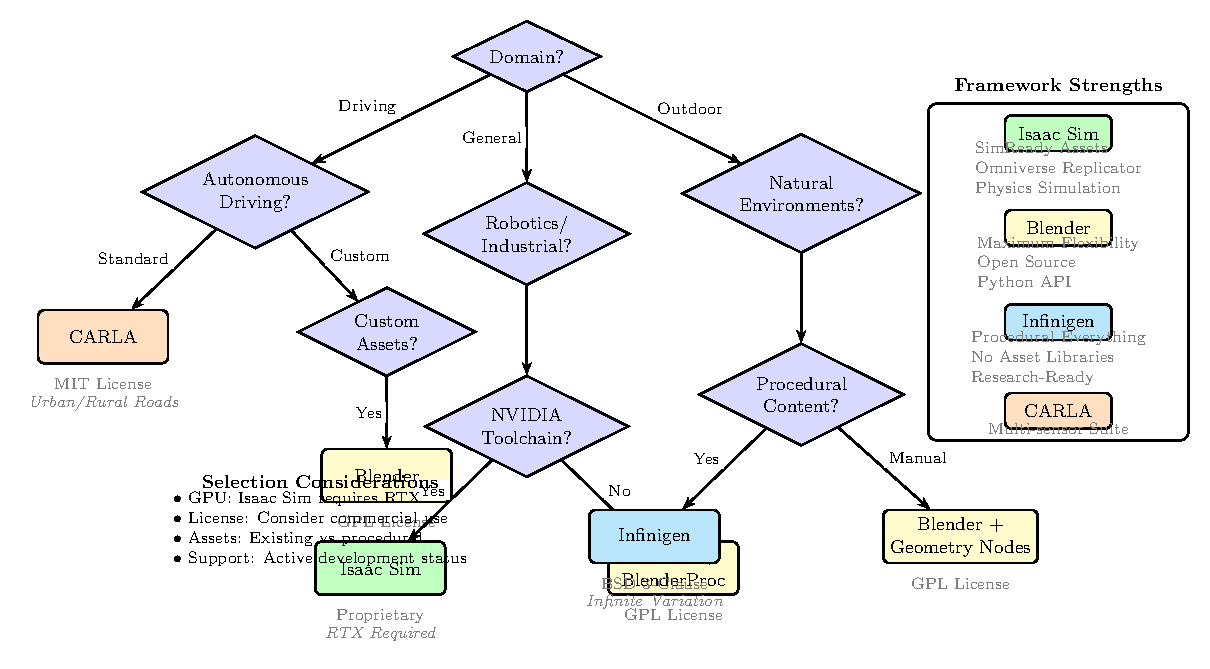
\includegraphics[width=\textwidth]{figures/ch04_fig4_framework_selection.pdf}
\caption{Decision tree for synthetic data generation framework selection. The tree guides practitioners through key decision points including application domain (driving, robotics, natural environments), integration requirements (NVIDIA toolchain compatibility), and content generation approach (procedural vs. asset-based). Framework strengths and licensing considerations are summarized in the accompanying reference panels.}
\label{fig:framework_selection}
\end{figure}

\section{Complete Parameter Taxonomy}
\label{sec:parameter_taxonomy}

This section presents an exhaustive taxonomy of tunable parameters for synthetic data generation, organized by functional category. For each parameter, we provide descriptions, typical ranges observed in the literature, and implementation considerations.

\begin{figure}[htbp]
\centering
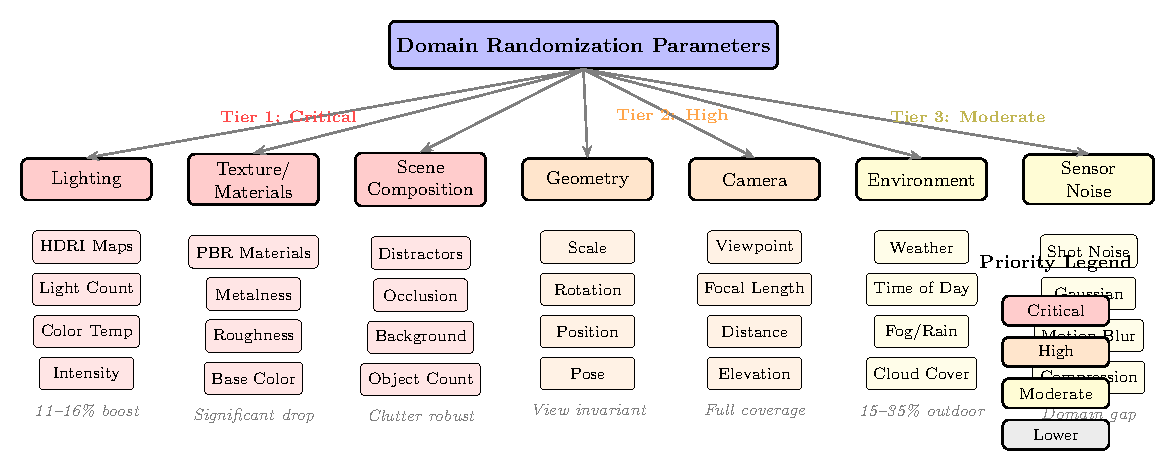
\includegraphics[width=\textwidth]{figures/ch04_fig2_parameter_taxonomy.pdf}
\caption{Hierarchical taxonomy of domain randomization parameters organized by priority tier. Tier 1 (Critical) parameters---lighting, texture/materials, and scene composition---demonstrate the largest impact on real-world detection performance. Tier 2 (High) parameters include geometry and camera settings. Tier 3 (Moderate) parameters cover environmental effects and sensor noise. Evidence-based impact annotations are shown below each parameter category.}
\label{fig:parameter_taxonomy}
\end{figure}

\subsection{Object Appearance Parameters}

Object appearance encompasses the visual properties of target objects and scene elements that determine their rendered appearance. These parameters directly influence the features that neural networks extract during training and are among the most critical for achieving robust real-world generalization.

\subsubsection{Texture Types}

Textures define the surface appearance of 3D objects and are typically implemented through one of three approaches. RGB textures assign uniform or randomly sampled color values to object surfaces, providing basic appearance variation with minimal computational overhead. This approach is commonly used in aggressive domain randomization where photorealism is sacrificed for maximum variation. Image-based textures apply photographic images to object surfaces through UV mapping, providing realistic surface detail at the cost of requiring texture asset libraries. Physically Based Rendering (PBR) textures represent the current state of the art, defining surface appearance through physically meaningful parameters including base color, metalness, roughness, and normal maps. Research has demonstrated that PBR materials produce superior results for reflective and metallic objects, with ablation studies showing significant performance drops when random textures are substituted for PBR materials.

\subsubsection{Material Properties}

Beyond texture mapping, material properties define how surfaces interact with light. Metalness, ranging from 0 (dielectric) to 1 (fully metallic), determines whether the surface exhibits diffuse reflection or metallic specular behavior. Roughness, also ranging from 0 to 1, controls the sharpness of specular reflections, with low values producing mirror-like reflections and high values producing diffuse highlights. Subsurface scattering simulates light penetration into translucent materials such as skin, wax, or vegetation. Index of refraction, typically ranging from 1.0 to 2.5, affects the intensity of specular reflections at grazing angles according to Fresnel equations.

\subsubsection{Color Variation Strategies}

Color variation may be implemented through several complementary strategies. Hue shifting rotates all colors in the image by a specified angular offset, typically limited to $\pm20$ degrees to maintain plausible appearances. Saturation adjustment scales color intensity between 0 (grayscale) and 150\% of original values. Value or brightness adjustment modifies overall luminance by $\pm30\%$. For object-specific variation, base colors may be sampled from predefined palettes that match the expected real-world color distributions for each object class.

Table~\ref{tab:appearance_params} summarizes the object appearance parameters with their typical ranges.

\begin{table}[htbp]
\centering
\caption{Object Appearance Parameters}
\label{tab:appearance_params}
\begin{tabular}{p{3.5cm}p{3cm}p{5cm}}
\hline
\textbf{Parameter} & \textbf{Typical Range} & \textbf{Implementation Notes} \\
\hline
Texture Type & RGB, Image, PBR & PBR preferred for reflective objects \\
Base Color & RGB [0,255] per channel & Sample from realistic color distributions \\
Metalness & [0.0, 1.0] & 0 for plastics, 1 for metals \\
Roughness & [0.0, 1.0] & 0.3--0.8 covers most real materials \\
Subsurface & [0.0, 1.0] & Enable for translucent materials \\
Index of Refraction & [1.0, 2.5] & 1.5 typical for glass and plastic \\
Normal Map Strength & [0.0, 2.0] & 1.0 is physically correct \\
Hue Shift & $[-20, +20]$ degrees & Larger shifts may appear unrealistic \\
Saturation Scale & [0.5, 1.5] & Maintain within plausible range \\
\hline
\end{tabular}
\end{table}

\subsection{Geometric Variation Parameters}

Geometric parameters control the spatial properties of objects including their size, orientation, and position. Adequate geometric variation is essential for training detectors that generalize across the range of object appearances expected in deployment.

\subsubsection{Scale Variations}

Scale variation simulates objects at different distances from the camera and natural variation in object size. Uniform scaling applies identical scale factors to all axes, typically ranging from 0.5$\times$ to 2.0$\times$ baseline size. Non-uniform scaling applies different factors per axis to simulate aspect ratio variation, typically constrained to 0.8$\times$ to 1.2$\times$ per axis to maintain object recognizability. Scale distributions should match the expected real-world size distribution, which may be obtained from domain knowledge or small real-world samples.

\subsubsection{Rotation Variations}

Rotation may be specified in Euler angles or quaternion representation. Full rotation covers all orientations with uniform sampling over SO(3), which is appropriate for objects without a natural upright orientation. Constrained rotation limits rotation to specified angular ranges, such as $\pm30$ degrees from upright, for objects that are typically observed in canonical orientations. Research has shown that appropriately constraining rotation based on domain knowledge improves detection performance compared to unrestricted rotation.

\subsubsection{Translation and Placement}

Object translation determines spatial position within the scene. Random placement samples positions uniformly within scene bounds but may produce unrealistic floating objects or interpenetrations. Physics-based placement enables objects to fall under gravity and settle on surfaces, producing realistic resting positions. Semantic placement positions objects according to functional relationships, such as dishes on tables or products on shelves.

\subsubsection{Pose Variation for Articulated Objects}

For articulated objects such as human figures, robotic arms, or animals, pose variation involves randomizing joint angles within their valid ranges. Each joint is typically parameterized by one to three rotation degrees of freedom with associated minimum and maximum angle limits. Pose sampling may be uniform within joint limits or weighted toward commonly observed configurations.

Table~\ref{tab:geometric_params} presents the complete geometric variation parameter set.

\begin{table}[htbp]
\centering
\caption{Geometric Variation Parameters}
\label{tab:geometric_params}
\begin{tabular}{p{3.5cm}p{3cm}p{5cm}}
\hline
\textbf{Parameter} & \textbf{Typical Range} & \textbf{Implementation Notes} \\
\hline
Uniform Scale & [0.5, 2.0] & Match expected distance variation \\
Per-Axis Scale & [0.8, 1.2] & Subtle aspect ratio variation \\
Rotation (Full) & [0, 360] all axes & Uniform sampling over SO(3) \\
Rotation (Constrained) & $\pm$30 degrees & Apply domain-appropriate limits \\
Translation X, Y & Scene bounds & Ensure object remains visible \\
Translation Z (Height) & [0, scene height] & Physics placement preferred \\
Joint Angles & Joint-specific limits & Valid kinematic configurations \\
\hline
\end{tabular}
\end{table}

\subsection{Scene Composition Parameters}

Scene composition determines the spatial arrangement of objects within the rendered environment, including object counts, occlusion relationships, and background content. These parameters have substantial impact on model robustness to cluttered real-world scenes.

\subsubsection{Object Density and Placement Strategies}

Object density specifies the number of target objects per rendered scene. Low density configurations with 1--3 objects simplify detection but may not prepare models for crowded scenarios. High density configurations with 10--20+ objects improve robustness to crowding but require careful management of occlusion levels. Placement strategies include uniform random sampling within scene bounds, grid-based placement with jittered positions, and constraint-based placement that respects spatial relationships.

\subsubsection{Occlusion Level Control}

Occlusion presents one of the most challenging aspects of real-world object detection, and synthetic data generation provides precise control over occlusion levels. Occlusion may be quantified as the percentage of object pixels visible (100\% minus occlusion percentage). Research categorizes occlusion into levels: no occlusion (100\% visibility), light occlusion (75--100\% visibility), moderate occlusion (50--75\% visibility), and heavy occlusion (25--50\% visibility). Training data should include examples across all occlusion levels with empirically determined distributions such as 40\% no occlusion, 30\% light, 20\% moderate, and 10\% heavy.

\subsubsection{Distractor Objects}

Distractor objects are non-target objects placed in scenes to increase visual complexity and train models to reject false positive detections. Research has demonstrated that including large numbers of distractor models, with studies using up to 15,000 unique distractors, improves detection robustness in cluttered environments. Distractors may be randomly selected from object databases such as Objaverse or domain-specific collections. The number of distractors per scene typically ranges from 0 to 50 depending on target scene complexity.

\subsubsection{Background Generation}

Background generation strategies significantly impact domain transfer. Random image backgrounds sample from large photographic databases such as ImageNet or Flickr to provide maximum appearance variation. Rendered 3D environments provide physically consistent backgrounds with proper lighting interaction. HDRI environment maps provide realistic 360-degree backgrounds captured from real locations. Research indicates that real photograph backgrounds composited behind rendered foreground objects improve sim-to-real transfer compared to purely synthetic backgrounds.

Table~\ref{tab:composition_params} summarizes scene composition parameters.

\begin{table}[htbp]
\centering
\caption{Scene Composition Parameters}
\label{tab:composition_params}
\begin{tabular}{p{3.5cm}p{3cm}p{5cm}}
\hline
\textbf{Parameter} & \textbf{Typical Range} & \textbf{Implementation Notes} \\
\hline
Target Object Count & [1, 20+] & Match expected scene density \\
Distractor Count & [0, 50] & Higher values for cluttered scenes \\
Occlusion Level & [0\%, 90\%] & Include distribution across levels \\
Placement Strategy & Random, Physics, Semantic & Physics-based most realistic \\
Background Type & Image, 3D, HDRI & Real photographs improve transfer \\
Scene Clutter Level & Low, Medium, High & Varies distractor density \\
Minimum Object Visibility & [10\%, 50\%] & Filter heavily occluded instances \\
\hline
\end{tabular}
\end{table}

\subsection{Lighting Parameters}

Lighting parameters control the illumination of synthetic scenes and represent one of the most impactful categories for detection performance. Research has consistently demonstrated that lighting variation during training substantially improves real-world generalization.

\subsubsection{Light Count and Configuration}

The number of light sources significantly affects scene appearance and shadow complexity. Single-light configurations produce hard, directional shadows while multi-light setups with 3--12 lights create more complex, realistic illumination. Point lights emit in all directions from a position in space. Area lights emit from a surface and produce soft shadows proportional to the light size. Directional lights simulate distant sources like the sun. Spot lights emit in a cone and are used for focused illumination.

\subsubsection{Light Position and Orientation}

Light positioning is typically specified in spherical coordinates relative to the scene center. Azimuth angle, ranging from 0 to 360 degrees, determines the horizontal direction. Elevation angle, ranging from 0 (horizon) to 90 (directly above), determines height. Distance affects intensity falloff. Full coverage of the hemisphere ensures the model sees objects illuminated from all directions.

\subsubsection{Intensity and Falloff}

Light intensity is specified in physically-based units such as watts or lumens, or in relative terms as a multiplier on baseline illumination. Intensity variation typically spans a 10$\times$ range on a logarithmic scale to cover dim indoor to bright outdoor conditions. Falloff follows inverse square law for physically accurate distance attenuation, though linear or constant falloff may be used for artistic control.

\subsubsection{Color Temperature}

Color temperature, measured in Kelvin, determines the spectral distribution of emitted light. Warm lighting at 2700--3500K matches incandescent sources and produces orange-yellow illumination. Neutral lighting at 4000--5000K matches daylight fluorescents. Cool lighting at 5500--6500K matches overcast daylight. Extended range up to 10000K covers blue sky illumination. Randomizing color temperature exposes models to the range of real-world illumination conditions.

\subsubsection{HDRI Environment Maps}

High Dynamic Range Image (HDRI) environment maps capture real-world lighting environments as 360-degree panoramic images with extended dynamic range. Each pixel stores both color and intensity for a specific direction, enabling physically accurate image-based lighting. Research has demonstrated that HDRI lighting produces an 11.11\% boost in classification accuracy and 16.04\% increase in AUC compared to simple directional lighting. HDRI databases such as Poly Haven provide hundreds of free environment maps covering indoor, outdoor, studio, and industrial settings.

\subsubsection{Shadow Characteristics}

Shadow appearance depends on light type and size. Point lights produce sharp shadows with hard edges. Area lights produce soft shadows with penumbra regions proportional to light size relative to occluder distance. Shadow density may be controlled by adjusting light intensities. Multiple lights create complex overlapping shadow patterns. Including shadow variation during training improves robustness to real-world lighting.

Table~\ref{tab:lighting_params} presents the complete lighting parameter set.

\begin{table}[htbp]
\centering
\caption{Lighting Parameters}
\label{tab:lighting_params}
\begin{tabular}{p{3.5cm}p{3cm}p{5cm}}
\hline
\textbf{Parameter} & \textbf{Typical Range} & \textbf{Implementation Notes} \\
\hline
Light Count & [1, 12] & Higher counts for complex illumination \\
Light Type & Point, Area, Directional & Mix types for realism \\
Position Azimuth & [0, 360] degrees & Full horizontal coverage \\
Position Elevation & [0, 90] degrees & Above-horizon positions \\
Intensity & [0.1, 10.0]$\times$ baseline & Log-scale sampling \\
Color Temperature & [2700, 10000] K & Match expected conditions \\
Area Light Size & [0.1, 2.0] meters & Affects shadow softness \\
Ambient Intensity & [0, 100]\% of total & Fills shadow regions \\
HDRI Environment & Database index & Randomize across collection \\
\hline
\end{tabular}
\end{table}

\subsection{Camera Parameters}

Camera parameters define the simulated imaging system, including optical properties and sensor configuration. Matching these parameters to the deployment camera improves domain transfer.

\subsubsection{Focal Length and Field of View}

Focal length, typically specified in 35mm equivalent millimeters, determines the field of view and perspective distortion characteristics. Wide-angle lenses with 18--35mm focal length capture more scene content but introduce perspective distortion. Normal lenses with 35--70mm approximate human vision. Telephoto lenses with 70--200mm compress perspective and narrow field of view. Field of view may alternatively be specified directly, typically ranging from 30 to 120 degrees.

\subsubsection{Lens Distortion Models}

Real camera lenses introduce geometric distortion that must be modeled for accurate synthetic data. Barrel distortion causes straight lines to curve outward from the image center. Pincushion distortion causes lines to curve inward. The Brown-Conrady model parameterizes distortion using radial coefficients $k_1$, $k_2$, $k_3$ and tangential coefficients $p_1$, $p_2$. Distortion parameters should be calibrated from the target deployment camera for maximum fidelity.

\subsubsection{Motion Blur Simulation}

Motion blur occurs when objects move relative to the camera during exposure. Object motion blur affects moving objects within the scene. Camera motion blur affects the entire image when the camera platform moves. Motion blur is typically specified by exposure time, with 0--50ms exposure producing varying degrees of blur depending on motion velocity. Motion blur should be included when training for detection of moving objects or from mobile platforms.

\subsubsection{Depth of Field}

Depth of field effects blur objects outside the focal plane. Aperture setting controls blur intensity, with wide apertures (low f-numbers like f/1.4) producing shallow depth of field and narrow apertures (high f-numbers like f/22) producing deep focus. For object detection, depth of field effects are typically disabled or minimized as they can obscure relevant image features. However, including moderate depth of field variation may improve robustness when deploying to cameras with limited hyperfocal capabilities.

Table~\ref{tab:camera_params} details camera parameters.

\begin{table}[htbp]
\centering
\caption{Camera Parameters}
\label{tab:camera_params}
\begin{tabular}{p{3.5cm}p{3cm}p{5cm}}
\hline
\textbf{Parameter} & \textbf{Typical Range} & \textbf{Implementation Notes} \\
\hline
Focal Length & [18, 200] mm & Match deployment camera \\
Field of View & [30, 120] degrees & Alternative to focal length \\
Camera Distance & [0.5, 5.0] meters & Determines object scale \\
Camera Azimuth & [0, 360] degrees & Full horizontal coverage \\
Camera Elevation & [-30, 90] degrees & Above and below horizon \\
Camera Roll & [-15, 15] degrees & Slight tilts only \\
Distortion $k_1$ & [-0.5, 0.5] & Calibrate from real camera \\
Distortion $k_2$ & [-0.2, 0.2] & Higher-order correction \\
Motion Blur & [0, 50] ms exposure & For dynamic scenarios \\
Aperture & f/1.4 to f/22 & Controls depth of field \\
\hline
\end{tabular}
\end{table}

\subsection{Environmental Parameters}

Environmental parameters simulate atmospheric and weather conditions that affect outdoor imagery. These parameters are essential for applications deployed in variable weather conditions.

\subsubsection{Weather Effects}

Rain simulation involves rendering falling droplets, wet surface reflections, and reduced visibility. Physics-based rain rendering adds realistic rain streaks and splashing effects. Research has demonstrated 15\% improvement in object detection and 35\% improvement in semantic segmentation when training includes rain-augmented data. Fog simulation reduces visibility through exponential or exponential-squared falloff with distance. Visibility distances typically range from 100m (dense fog) to 10km (light haze). Snow simulation combines falling particles with ground accumulation and reduced visibility.

\subsubsection{Time of Day Simulation}

Time of day determines sun position and color, sky appearance, and overall scene illumination. Solar position is calculated from geographic location and time. Dawn and dusk produce warm, directional illumination with long shadows. Midday produces harsh overhead illumination. Night requires artificial lighting sources. Sky color transitions from warm oranges at horizon to deep blues at zenith during golden hour.

Table~\ref{tab:environmental_params} presents environmental parameters.

\begin{table}[htbp]
\centering
\caption{Environmental Parameters}
\label{tab:environmental_params}
\begin{tabular}{p{3.5cm}p{3cm}p{5cm}}
\hline
\textbf{Parameter} & \textbf{Typical Range} & \textbf{Implementation Notes} \\
\hline
Time of Day & [0, 24] hours & Affects sun position and color \\
Cloud Cover & [0, 100]\% & Affects diffuse lighting \\
Rain Intensity & [0, 100] mm/hr & Include streaks and puddles \\
Fog Visibility & [100, 10000] meters & Exponential falloff model \\
Snow Intensity & Light, Medium, Heavy & Combine with fog \\
Wet Surface & Dry, Wet, Puddled & Increases specularity \\
Wind Speed & [0, 30] m/s & Affects vegetation motion \\
\hline
\end{tabular}
\end{table}

\subsection{Sensor Noise Parameters}

Sensor noise parameters simulate the imperfections inherent in real camera systems. Appropriate noise modeling is critical for bridging the domain gap between synthetic and real imagery.

\subsubsection{Gaussian Noise}

Additive white Gaussian noise (AWGN) represents random intensity variations independent of signal level. Gaussian noise is characterized by its standard deviation $\sigma$, typically ranging from 0 to 25 on an 8-bit [0, 255] scale. While AWGN is commonly used for its simplicity, it does not accurately represent real camera noise, which is signal-dependent.

\subsubsection{Shot Noise}

Shot noise, also called photon noise, arises from the discrete nature of photon arrivals at the sensor. Shot noise follows a Poisson distribution where variance equals the mean signal level, causing brighter regions to exhibit more noise than darker regions. Physics-based shot noise simulation improves realism compared to uniform Gaussian noise.

\subsubsection{Salt-and-Pepper Noise}

Salt-and-pepper noise simulates sensor defects that cause pixels to read at maximum (white) or minimum (black) values. The noise is characterized by the probability of pixel corruption, typically ranging from 0 to 5\%. This noise type simulates dead pixels and transmission errors.

\subsubsection{ISO Simulation}

ISO setting on real cameras controls sensor sensitivity by adjusting analog and digital gain. Higher ISO values amplify both signal and noise, increasing image brightness at the cost of increased noise visibility. ISO simulation typically ranges from 100 (low noise) to 12800 (high noise), with noise characteristics varying based on the simulated sensor model.

\subsubsection{Compression Artifacts}

JPEG and video compression introduce blocking artifacts, ringing around edges, and color quantization. Compression quality settings from 50\% (heavy compression) to 100\% (minimal compression) control artifact severity. Including compression artifacts in training data improves robustness when deploying to systems with compressed video pipelines.

Table~\ref{tab:noise_params} summarizes sensor noise parameters.

\begin{table}[htbp]
\centering
\caption{Sensor Noise Parameters}
\label{tab:noise_params}
\begin{tabular}{p{3.5cm}p{3cm}p{5cm}}
\hline
\textbf{Parameter} & \textbf{Typical Range} & \textbf{Implementation Notes} \\
\hline
Gaussian $\sigma$ & [0, 25] 8-bit scale & Simple but not realistic \\
Shot Noise & Signal-dependent & Poisson model preferred \\
Salt-and-Pepper & [0, 5]\% pixels & Simulate sensor defects \\
Read Noise & Camera-specific & From sensor datasheet \\
Dark Current & Temperature-dependent & Low priority \\
ISO Equivalent & [100, 12800] & Higher = more noise \\
JPEG Quality & [50, 100]\% & For compressed pipelines \\
\hline
\end{tabular}
\end{table}

\section{Parameter Priority Ranking}
\label{sec:priority_ranking}

This section presents an evidence-based ranking of parameter importance derived from ablation studies and empirical research in the synthetic data generation literature. Understanding parameter priority enables efficient allocation of effort and computational resources during synthetic dataset construction.

\subsection{Tier 1: Critical Impact Parameters}

Tier 1 parameters have demonstrated the largest impact on real-world detection performance in controlled experiments. These parameters should receive priority attention in any synthetic data generation pipeline.

Dataset diversity and scale represents the most impactful factor overall. Research on YOLOv11 demonstrated that expanding the dataset with varied viewpoints and negative examples outperformed augmentation techniques applied to a smaller base dataset. The inclusion of images without target objects (negative examples) proved essential for reducing false positive rates in deployment.

Lighting variation consistently ranks among the most critical parameters. HDRI environment lighting produced 11.11\% improvement in classification accuracy compared to simple directional lighting. Multi-light configurations with randomized positions, intensities, and color temperatures ensure exposure to the range of illumination conditions encountered in real environments.

Object texture and material properties demonstrate substantial impact, particularly for reflective or metallic objects. Ablation studies found that excluding random textures or reducing texture variants resulted in significant performance drops. PBR materials that accurately model surface reflectance outperform simple RGB color assignments.

Background and scene composition directly impacts the model's ability to distinguish target objects from visual clutter. Real photograph backgrounds improve domain transfer compared to purely synthetic backgrounds. Including diverse distractor objects, with research using up to 15,000 unique distractor models, trains models to reject false positive detections.

Camera viewpoint variation ensures the model observes objects from all angles. Full azimuth coverage (0--360 degrees) and broad elevation coverage (-30 to +90 degrees) are necessary for viewpoint-invariant detection.

\subsection{Tier 2: High Impact Parameters}

Tier 2 parameters have demonstrated meaningful impact on detection performance and should be included when computational resources permit.

Occlusion level variation trains models to detect partially visible objects. Including examples across occlusion levels from 0\% to 75\% improves robustness to real-world scenarios where objects are frequently partially hidden.

Object scale variation prepares models for objects at different distances. Wide scale ranges (0.5$\times$ to 2.0$\times$ baseline) are necessary to match the range of apparent object sizes in deployment.

Rendering quality, specifically the choice between path tracing and rasterization, produces measurable differences. Path tracing consistently outperforms rasterization by 0.3\% to 5.1\% mAP@50, justifying the additional rendering time for critical applications.

Post-processing noise and blur, when appropriately calibrated, improve domain transfer. Ablation studies found that removing noise and blur effects caused performance drops, particularly in robotics and industrial applications.

Object rotation and pose variation ensures the model recognizes objects across their range of possible orientations. Constraints should be applied based on domain knowledge of expected object configurations.

\subsection{Tier 3: Moderate Impact Parameters}

Tier 3 parameters provide incremental improvements and should be included when sufficient resources are available.

Weather effects including rain, fog, and snow are essential for outdoor applications but may be omitted for controlled indoor environments. Research demonstrated 15--35\% improvement on weather-degraded test images when weather augmentation was included during training.

Color and brightness jitter through standard image augmentation provides moderate improvement with minimal computational cost. These augmentations are typically applied during training data loading rather than during rendering.

Distractor object diversity beyond baseline levels provides diminishing returns. While some distractor objects are essential (Tier 1), maximizing distractor variety provides incremental benefit.

Compositional augmentation techniques such as Mixup and Mosaic, applied during training, improve performance on cluttered scenes. These techniques combine multiple training images to create synthetic crowded scenarios.

\subsection{Tier 4: Lower Priority Parameters}

Tier 4 parameters provide minimal impact in most scenarios and may be omitted to reduce pipeline complexity.

Lens distortion modeling is necessary only when the deployment camera exhibits significant geometric distortion. For well-corrected lenses, distortion simulation provides minimal benefit.

Motion blur is relevant only for applications involving moving cameras or fast-moving objects. For static scene detection, motion blur may actually degrade performance.

Chromatic aberration produces subtle color fringing that is rarely visible in typical imaging conditions. The impact on detection performance is minimal.

Compression artifacts should be included when training for compressed video pipelines but may be omitted for uncompressed image detection.

Depth of field effects are generally not beneficial for detection tasks, as blur obscures object features. This effect should be minimized or disabled.

Table~\ref{tab:priority_ranking} summarizes the parameter priority ranking with supporting evidence.

\begin{table}[htbp]
\centering
\caption{Parameter Priority Ranking with Evidence}
\label{tab:priority_ranking}
\begin{tabular}{p{1cm}p{3.5cm}p{6cm}}
\hline
\textbf{Tier} & \textbf{Parameter Category} & \textbf{Evidence Summary} \\
\hline
1 & Dataset Diversity & Expanded datasets with negatives outperform augmentation \\
1 & Lighting Variation & HDRI: 11--16\% improvement over simple lighting \\
1 & Texture/Materials & Excluding textures causes significant performance drop \\
1 & Scene Composition & Distractors essential for clutter robustness \\
1 & Camera Viewpoint & Full coverage necessary for invariance \\
\hline
2 & Occlusion Levels & Trains for partially visible object detection \\
2 & Object Scale & Addresses distance variation \\
2 & Path Tracing & 0.3--5.1\% mAP improvement over rasterization \\
2 & Noise/Blur & Removing causes performance drops \\
2 & Rotation/Pose & Enables orientation invariance \\
\hline
3 & Weather Effects & 15--35\% improvement on degraded images \\
3 & Color Jitter & Standard augmentation, moderate impact \\
3 & Distractor Diversity & Diminishing returns beyond baseline \\
3 & Mixup/Mosaic & Helps with cluttered scenes \\
\hline
4 & Lens Distortion & Only for distorted deployment cameras \\
4 & Motion Blur & Only for dynamic scenarios \\
4 & Chromatic Aberration & Minimal visible impact \\
4 & Compression Artifacts & Only for compressed pipelines \\
4 & Depth of Field & Generally not beneficial \\
\hline
\end{tabular}
\end{table}

\section{Generation Pipeline Architecture}
\label{sec:pipeline_architecture}

This section describes the end-to-end architecture for synthetic data generation pipelines, including annotation format generation for YOLO training and quality control measures.

\subsection{End-to-End Pipeline Design}

A complete synthetic data generation pipeline comprises several interconnected stages: scene assembly, parameter sampling, rendering, annotation extraction, and quality validation. The following algorithmic description presents a generalized pipeline architecture applicable across rendering frameworks.

\begin{algorithm}
\caption{Synthetic Data Generation Pipeline}
\label{alg:sdg_pipeline}
\begin{algorithmic}[1]
\Require Asset library $\mathcal{A}$, parameter distributions $\mathcal{D}$, target count $N$
\Ensure Dataset $\{(I_i, A_i)\}_{i=1}^N$ of images and annotations
\State Initialize rendering engine and scene
\For{$i = 1$ to $N$}
    \State Clear scene of previous objects
    \State Sample parameters $\theta \sim \mathcal{D}$ \Comment{All parameter categories}
    \State Configure lighting from $\theta_{\text{light}}$
    \State Configure camera from $\theta_{\text{camera}}$
    \State Place target objects with $\theta_{\text{object}}$
    \State Place distractor objects with $\theta_{\text{distractor}}$
    \State Configure materials from $\theta_{\text{appearance}}$
    \State Apply environmental effects from $\theta_{\text{environment}}$
    \State $I_i \gets$ \Call{Render}{scene}
    \State $A_i \gets$ \Call{ExtractAnnotations}{scene, format=YOLO}
    \State Apply post-processing noise from $\theta_{\text{noise}}$
    \If{\Call{PassesQualityChecks}{$I_i$, $A_i$}}
        \State Save $(I_i, A_i)$ to dataset
    \Else
        \State Decrement $i$ \Comment{Regenerate failed sample}
    \EndIf
\EndFor
\State \Return Dataset
\end{algorithmic}
\end{algorithm}

The pipeline begins by initializing the rendering engine and loading the base scene template. For each sample, the scene is cleared and fresh parameters are sampled from the specified distributions. Scene elements are configured in order of decreasing spatial extent: first the environment and lighting, then camera placement, then object placement and materials. This ordering ensures that dependent parameters, such as camera framing that depends on object positions, can be computed correctly.

Rendering produces the RGB image along with auxiliary passes that enable annotation extraction. Common auxiliary passes include object indices (enabling segmentation and bounding box extraction), depth (enabling 3D reasoning), and surface normals (useful for pose estimation). After rendering, post-processing effects such as noise and blur are applied as image-space operations.

Quality checks verify that generated samples meet minimum requirements before inclusion in the dataset. Failed samples are discarded and regenerated to maintain dataset quality without introducing bias toward easy configurations.

\subsection{Annotation Format Generation}

YOLO format annotations consist of text files with one line per object, containing class index and normalized bounding box coordinates. The format specification requires coordinates in the form (class, x\_center, y\_center, width, height) where all spatial values are normalized to [0, 1] relative to image dimensions.

\begin{algorithm}
\caption{YOLO Annotation Extraction}
\label{alg:yolo_annotation}
\begin{algorithmic}[1]
\Require Scene graph $S$, image dimensions $(W, H)$, class mapping $C$
\Ensure YOLO format annotation string
\State annotations $\gets$ empty list
\For{each object $o$ in $S$.target\_objects}
    \State $\text{bbox} \gets$ \Call{GetBoundingBox}{$o$} \Comment{In pixels}
    \State $x_{\min}, y_{\min}, x_{\max}, y_{\max} \gets \text{bbox}$
    \State $x_c \gets (x_{\min} + x_{\max}) / (2 \cdot W)$ \Comment{Normalize}
    \State $y_c \gets (y_{\min} + y_{\max}) / (2 \cdot H)$
    \State $w \gets (x_{\max} - x_{\min}) / W$
    \State $h \gets (y_{\max} - y_{\min}) / H$
    \State class\_id $\gets C[o.\text{class\_name}]$
    \State Append ``class\_id $x_c$ $y_c$ $w$ $h$'' to annotations
\EndFor
\State \Return Join annotations with newlines
\end{algorithmic}
\end{algorithm}

Bounding box extraction from rendered scenes leverages the rendering engine's ability to identify object pixels. In Blender, this is accomplished using the IndexOB pass which assigns unique integer values to each object. The bounding box is computed as the axis-aligned extent of all pixels belonging to each object. Objects that are completely occluded (zero visible pixels) are excluded from annotations. Partially occluded objects may be included with their full extent or with visible-only extent depending on annotation policy.

The dataset directory structure follows YOLO conventions with separate directories for images and labels. Training, validation, and test splits are organized into subdirectories. A data.yaml file specifies paths and class names for the dataset.

\subsection{Quality Control Measures}

Quality control ensures that generated samples meet minimum standards for training utility. Several automated checks should be applied to each generated sample.

Minimum object visibility requires that target objects have at least some percentage (typically 10--25\%) of their pixels visible in the rendered image. Completely occluded objects provide no training signal and should be excluded from annotations or the sample regenerated.

Object visibility verification confirms that at least one target object is present and visible in each sample, unless the sample is explicitly designated as a negative example. The balance between positive and negative samples should be monitored to maintain desired ratios.

Bounding box validation confirms that extracted bounding boxes fall within image bounds and have non-zero area. Degenerate boxes indicate extraction errors or edge cases that should be filtered.

Image quality metrics may be computed to detect rendering failures. Metrics include checking for completely black or white images (rendering failures), extremely low or high average brightness (lighting configuration errors), and presence of expected color distributions.

Annotation consistency verification confirms that the number of annotations matches the expected object count and that class labels are valid. Mismatches may indicate scene configuration errors or extraction bugs.

\subsection{Pipeline Architecture Diagram}

Figure~\ref{fig:pipeline_diagram} illustrates the complete synthetic data generation pipeline architecture.

\begin{figure}[htbp]
\centering
\begin{tikzpicture}[
    node distance=1.5cm and 2cm,
    box/.style={rectangle, draw, minimum width=2.5cm, minimum height=1cm, align=center, fill=blue!10},
    data/.style={rectangle, draw, minimum width=2cm, minimum height=0.8cm, align=center, fill=green!10},
    arrow/.style={->, >=stealth, thick}
]

\node[box] (params) {Parameter\\Sampler};
\node[box, right=of params] (scene) {Scene\\Assembly};
\node[box, right=of scene] (render) {Rendering\\Engine};
\node[box, below=of render] (postproc) {Post-\\Processing};
\node[box, left=of postproc] (annotate) {Annotation\\Extraction};
\node[box, left=of annotate] (validate) {Quality\\Validation};

\node[data, above=0.8cm of params] (config) {Configuration\\$\mathcal{D}$};
\node[data, above=0.8cm of scene] (assets) {Asset\\Library};
\node[data, below=0.8cm of validate] (dataset) {YOLO\\Dataset};

\node[box, below=of validate, xshift=-2cm] (rl) {RL\\Controller};

\draw[arrow] (config) -- (params);
\draw[arrow] (assets) -- (scene);
\draw[arrow] (params) -- (scene);
\draw[arrow] (scene) -- (render);
\draw[arrow] (render) -- (postproc);
\draw[arrow] (postproc) -- (annotate);
\draw[arrow] (annotate) -- (validate);
\draw[arrow] (validate) -- (dataset);

\draw[arrow, dashed] (rl.north) -- ++(0, 0.5) -| (params.south);
\draw[arrow, dashed] (dataset.south) -- ++(0, -0.5) -| (rl.east);

\node[below=0.3cm of rl, align=center, font=\small] {Reward: mAP\\on validation set};

\end{tikzpicture}
\caption{Synthetic data generation pipeline architecture with optional reinforcement learning parameter optimization. Solid arrows indicate data flow during generation. Dashed arrows indicate the RL feedback loop where real-world validation performance guides parameter distribution updates.}
\label{fig:pipeline_diagram}
\end{figure}

The architecture supports optional integration of reinforcement learning for parameter optimization. In this configuration, the RL controller adjusts parameter distributions based on feedback from model performance on a held-out real-world validation set. The reward signal, typically mAP@50 or similar detection metrics, guides the search toward parameter configurations that maximize sim-to-real transfer. This approach has been demonstrated to achieve superior results compared to hand-tuned parameter distributions.

\subsection{Computational Considerations}

Rendering time dominates the computational cost of synthetic data generation. Path tracing produces higher quality images but requires substantially more time than rasterization. GPU acceleration through NVIDIA RTX ray tracing cores or CUDA-accelerated rendering significantly improves throughput.

Typical rendering times per image range from 0.5--2 seconds for rasterization at 1080p resolution to 10--60 seconds for converged path tracing depending on scene complexity and sample count. A dataset of 10,000 images may thus require 1--150 hours of rendering time, making parallelization across multiple GPUs essential for large-scale dataset generation.

Memory requirements depend on scene complexity, texture resolution, and rendering resolution. Complex scenes with high-resolution PBR textures may require 8--16 GB of GPU memory. Batch rendering can amortize scene loading overhead when generating many variations of similar scenes.

Storage requirements for synthetic datasets are comparable to real image datasets. A 10,000 image dataset at 1080p with JPEG compression requires approximately 5--10 GB. Including auxiliary passes (depth, normals, segmentation) increases storage by 2--4$\times$.

\section{Summary}

This chapter has provided a comprehensive treatment of synthetic data generation for object detection training. The major frameworks including NVIDIA Isaac Sim, Blender, Infinigen, Unity Perception, and CARLA each offer distinct capabilities suited to different application domains. The complete parameter taxonomy spans object appearance, geometry, scene composition, lighting, camera, environment, and sensor noise, with each category containing multiple tunable parameters that influence detection performance.

The evidence-based priority ranking identifies lighting variation, texture diversity, scene composition, and viewpoint coverage as the most critical parameters for real-world generalization. Path tracing rendering, appropriate noise modeling, and comprehensive occlusion variation comprise the second tier of importance. Weather effects and advanced augmentation techniques provide incremental improvements, while lens distortion and motion blur are relevant only for specific deployment scenarios.

The generation pipeline architecture integrates parameter sampling, scene assembly, rendering, annotation extraction, and quality validation into a cohesive system capable of producing YOLO-compatible datasets. Optional reinforcement learning integration enables automated optimization of parameter distributions based on real-world validation performance, potentially surpassing manually tuned configurations.

Practitioners should prioritize matching deployment camera characteristics, including diverse negative examples, and validating exclusively on real-world data rather than synthetic hold-out sets. The synthetic validation metrics can be misleadingly optimistic, with studies reporting near-perfect synthetic validation mAP while real-world performance remains substantially lower. This domain gap underscores the importance of the parameter randomization and quality control strategies presented in this chapter.
